\section*{Formal Definition}
	Formally, a network or graph is a mathematical object consisting of sets of edges (arcs) and nodes (vertices), which can be written as $G = (E,V)$. In many cases, an \textit{adjacency matrix} is used as a representation of a network, where each element of the matrix $A_{ij}$ takes a binary value, $1$ for presence of an edge between nodes $i$ and $j$, and $0$ if there is no edge between these nodes. The network having binary values for edges is called an \textit{unweighted} networks  If the matrix is symmetric, namely $A_{ij} = A_{ji},  \forall i,j \in V$, the matrix represents an \textit{undirected} network in which edges do not have directionality at all. If the matrix is asymmetric, on the other hand, it's representing a \textit{directed} network, where an element $A_{ij}$ implies an edge originating from the node $i$ and pointing to the node $j$. If edges of the network are weighted, meaning that edges can have real values, then the network is called \textit{weighted}. Related with weighted networks is \textit{multigraph} in which any pair of nodes is allowed to have multiple edges connecting them. One should be careful here with the representation with an adjacency matrix for weighted network and multigraph, as the interpretation of the value of $A_{ij}$ depends on the context in which one treats the graph for the problem. For example, $A_{ij} = 2$ may describe an edge between $i$ and $j$ weighted by $2$, or it may represent \textit{two} edges running between $i$ and $j$. If diagonal elements of a matrix $A$ are non-zero, the network has \textit{self-loops} which indicates that there are edges originating from and pointing to the exact same node. In many studies such self-loops are simply ignored for the sake of simplicity. The last, but not the least kind of network is \textit{bipartite network}, in which there are two groups of nodes and edges exist \textit{only} between nodes of different groups. An example of bipartite network is a network of cooperate board membership where there are groups of companies and board members and edges connect companies and board members. Often times, a bipartite network is converted into a network in which there is only one kind of nodes, for instance only board members in the case of cooperate board membership network, by an operation called one-mode projection. In the one-mode projected network of board members, an edge between persons $i$ and $j$ now represents the frequency that they sit on the same board for companies.
	
	As such, there are many kinds of networks, each describing networks differently. In our study, for the sake of simplicity and comparability, we focus on using a \textit{simple graph}, in which edges have no directionality and weight and there is no self-loops. A set of procedures for converting non-simple graphs into simple graphs is defined as follows:
	
	\begin{enumerate}
		\item if a network is directed, then discard the directionality.
		\item If a network is weighted, then convert any non-zero weight into $1$ and $0$ otherwise.
		\item If a network is multigraph, namely having multiple edges between a pair of nodes, then merge them into one edge.
		\item if a network contains self-loops, then discard them.
	\end{enumerate}
	
	\subsection*{Structural Features of A Network}
	There are many ways to characterize a network in a quantitative manner that use the network's structural features \cite{Newman:NetworksIntro,NetworkCharacterizationSurvey}. Some network features, however, are implicitly correlated with the size of networks, which itself is a very strong feature: the number of nodes in web graphs is usually a magnitude of $10^6$ or more whereas ecological food webs contain usually less than 100 nodes. Examples of such features include, for instance, distance-related features such as the average path length and network diameter that are believed to grow approximately in $O(\log n)$, where $n$ is the number of nodes in a network. Another structural feature correlated with the size of the network is the modularity of network \cite{Modularity1}. Simply put, modularity quantifies the degree to which how much an observed network can be "partitioned" into modules within which edges are densely present but between which edges are sparsely present. The derivation of modularity is essentially based on comparing the original network with a random network having the same degree distribution which is called the configuration model and the value of modularity is practically the degree of difference between the original graph and its randomized counterpart. If the size of a network is large, the random network becomes so different that the modularity value becomes large as well \cite{ResolutionLimit, ModularityLimit}.
	
	The feature set we use in this study is scale-invariant, meaning that the size of network does not affect the value of a feature. This set of features allows us to compare networks without the notion of network size. In the following sections we describe important structural features that are relevant in this study.	
	 
\subsection*{Degree}
	The \textit{degree} of a node in a network is the number of edges attached to the node. For a node $i$ in an unweighted network, the degree $k_i$ of the node can be written mathematically as:
	
	\begin{equation}
 	 k_i = \sum_{j = 1}^n A_{ij}.
	\end{equation}

	
\subsection*{Clustering Coefficient}
	Clustering coefficient, which describes a degree of \textit{transitivity} in a network, is one of the most widely used metrics in network analysis especially in the context of social network. Transitivity in the context of networks means that if nodes $a$ and $b$ are connected as well as nodes $b$ and $c$, then nodes $a$ and $c$ are connected. Mathematically, the definition of clustering coefficient of a network is given by the following equation:
	\begin{equation}
	C = \frac{\text{number of closed paths of length two}}{\text{number of paths of length two}}.
	\end{equation}
	

\subsection*{Degree Assortativity}
	\textit{Assortativity} in a network indicates a tendency for nodes to be connected to other nodes with similar node attribute. In a social network, for instance, node attributes which could be the basis for assortativity include language, age, income, alma mater, etc. On the other hand, \textit{disassortativity} exhibits nodes' tendency to be connected to other nodes having different node attribute in the network. An example network of disassortatvity would be a social network of heterosexual-relationship among people. 
	\textit{Degree assortativity} is a form of assortativity in which nodes with similar degree value tend to be connected together. Therefore in a network exhibiting high degree assortativity, there is a core of highly connected nodes with the high degree and periphery of nodes sparsely connected to other low-degree nodes.
	
	Here, we first define the covariance of $x_i$ and $x_j$ for the vertices at the ends of all edges, which leads us to a general \textit{assortativity coefficient}:
	
	\begin{equation}
		\text{cov}(x_i, x_j) = \frac{1}{2m}\sum_{ij}(A_{ij} - \frac{k_i k_j}{2m})x_i x_j,				
	\end{equation}
where $x_i$,$x_j$ are nodes $i$ and $j$'s attributes. This covariance will be positive if both $x_i$ and $x_j$ have, in average, similar values, and will be negative if both $x_i$ and $x_j$ tend to change in a different direction. We normalized cov($x_i$,$x_j$) by another quantity which represents a perfect assortativity, so that it takes a value $r \in [-1 ,1]$. The perfect matching happens if $x_i = x_j$ for all edges, and cov($x_i$,$x_i$) becomes:
	\begin{equation}
	\begin{split}
	 \text{cov}(x_i, x_i) &=  \frac{1}{2m}\sum_{ij}(A_{ij} x_i^2 - \frac{k_i k_j}{2m} x_i x_j) \\
	 		             &=  \frac{1}{2m}\sum_{ij}(k_i \delta_{ij} - \frac{k_i k_j}{2m}) x_i x_j,
	\end{split}
	\end{equation}
	where $\delta_{ij}$ is Kronecker delta.
Thus, the normalized covariance becomes as follows:
	\begin{equation}
	\begin{split}
	 r = \frac{ \text{cov}(x_i, x_j)}{ \text{cov}(x_i, x_i)} = 
	 \cfrac{\sum_{ij}(A_{ij} - \cfrac{k_i k_j}{2m})x_i x_j}{\sum_{ij}(k_i \delta_{ij} - \cfrac{k_i k_j}{2m}) x_i x_j}.
	\end{split}
	\end{equation}

Degree assortativity coefficient can easily be obtained by substituting $x_i$ and $x_j$ with degrees of respective vertices, thus:
	\begin{equation}
	 r =  \cfrac{\sum_{ij}(A_{ij} - \cfrac{k_i k_j}{2m})k_i k_j}{\sum_{ij}(k_i \delta_{ij} - \cfrac{k_i k_j}{2m}) k_i k_j}.
	\end{equation}

\subsection*{Network Motifs} 
The idea of \textit{network motifs} was first introduced by Milo \textit{et al.} \cite{Milo_motif}. A network motif is a sub-graph of a network that appears more statistically significant than in random networks having the same degree distribution, namely the configuration model. There are a number of studies using network motifs of directed networks, where edges have directions, especially in biological sciences \cite{Alon2007, MotifsInBrain, NetworkMotifsEcoli}. Biologists have been particularly interested in motifs of networks, such as gene regulatory networks, since they are thought to correspond to the functional building blocks in biological systems and may help scientists understand the underlying principles of biological complex systems.
As opposed to the number of studies using directed network motifs, in this study we only use network motifs of undirected networks, that produce fewer variations in motif kinds, but can be applied to any network regardless of edge directionality which is crucial for our study. Fig.~\ref{motifs} shows the complete list of $k=4$ undirected connected subgraphs used in this study.

\begin{figure}[ht]
	\begin{center}
		\vspace{0.5cm}
		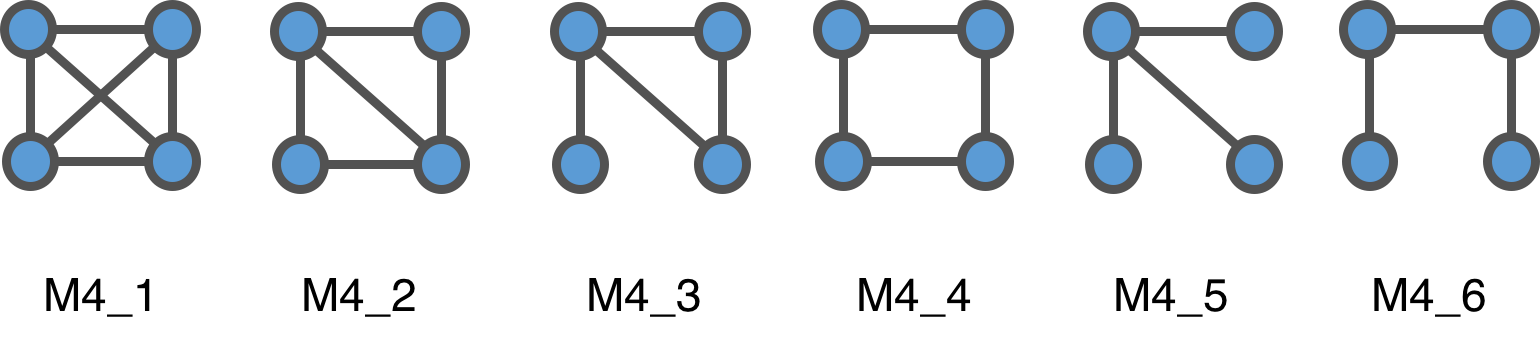
\includegraphics[clip,width=7cm,height = 2cm]{figs/motifs.png}
		\vspace{0.5cm}
		\caption{Undirected subgraphs of $k =4$, where $k$ is the number of nodes.}
		\label{motifs}
	\end{center}
\end{figure}

In order to quantify network motifs, we first count the occurrence of each sub-graph in the original network, then repeat the same process on the configuration models. After counting occurrences of sub-graphs in both original and multiple random networks, we proceed to calculate z-score for each sub-graph $i$ as follows:
	\begin{equation}
	Z_i = \cfrac{N_i^{\text{original}} - \langle N_i^{\text{random}} \rangle }{\sigma_i^{\text{random}}},
	\end{equation}

where $N_i^{\text{original}}$ is the number of occurrence of a sub-graph $i$ in the original network and $ \langle N_i^{\text{random}} \rangle$ and $\sigma_i^{\text{random}}$ are the average and the standard deviation of the number of occurrence of a sub-graph $i$ in an ensemble of random networks. It is usually convenient to normalize this z-score as some networks exhibits very large values due to the size of the networks. Such normalized z-score is called \textit{significance profile} and is defined as follows:
	\begin{equation}
	SP_i = \cfrac{Z_i}{\sum_j Z_j^2}.
	\end{equation}
	
In this study, we treat the significance profile for each subgraph as a feature and in total we have six features as network motifs.
\newline


\begin{table}[htb]
  %\begin{center}
    \caption{Network Features.}
    %\begin{tabular}{| l | p{5cm} |} \hline
    \begin{tabular}{| p{3cm} | p{5cm} |} \hline
      Name of the feature & Explanation  \\ \hline \hline
      Clustering coefficient &  The probability that a connected triplet ($k=3$ subgraph) is a triangle \\  %\hline
      Degree assortativity &  Correlation between a pair of connected nodes' degree. \\  %\hline
      Network motifs & The normalized z score of a subgraph's frequency compared to that of an ensemble of random networks having the exact same degree distribution. \\ \hline
    \end{tabular}
    \label{tab:feature}
  %\end{center}
\end{table}
